\subsection{\texorpdfstring{\(E_{6}\) 型系统}{E\_6 型系统}}

\begin{enumerate}
\def\labelenumi{(\Roman{enumi})}
\tightlist
\item
  以及 (II) 设 \(E = R^{8}\) ，并令 \(R_{8}\) 为第 10 号中构造的 E 中的根系。令 V 为 E 中由根 \(\alpha_{1}, \ldots, \alpha_{6}\)（属于 \(R_{8}\)）所生成的向量子空间；它是由最后两个基本权 \(\omega = \varepsilon_{7} + \varepsilon_{8}\) 和 \(\pi = \varepsilon_{6} + \varepsilon_{7} + 2\varepsilon_{8}\)（属于 \(R_{8}\)）所生成平面的正交补。
\end{enumerate}

令 \(R = R_{8} \cap V\) 。这是一个以 \((\alpha_{1}, \ldots, \alpha_{6})\) 为基的约化根系，因而是 \(E_{6}\) 型的根系。其元素为：

\[
\begin{array}{c} \pm \varepsilon_ {i} \pm \varepsilon_ {j} (1 \leqslant i <   j \leqslant 5), \\ \pm \frac {1}{2} (\varepsilon_ {8} - \varepsilon_ {7} - \varepsilon_ {6} + \sum_ {i = 1} ^ {5} (- 1) ^ {\nu (i)} \varepsilon_ {i}) \text {with} \sum_ {i = 1} ^ {5} \nu (i) \text {even.} \end{array}
\]

根的数目为 \(n = \binom{5}{2}.4 + 2^5 = 72\) 。正根为

\[
\pm \varepsilon_ {i} + \varepsilon_ {j} (1 \leqslant i <   j \leqslant 5),
\]

\[
\frac {1}{2} \left(\varepsilon_ {8} - \varepsilon_ {7} - \varepsilon_ {6} + \sum_ {i = 1} ^ {5} (- 1) ^ {\nu (i)} \varepsilon_ {i}\right) \text {with} \sum_ {i = 1} ^ {5} \nu (i) \text {even}.
\]

\begin{enumerate}
\def\labelenumi{(\Roman{enumi})}
\setcounter{enumi}{2}
\item
  我们有 \(h = \frac{n}{6} = 12\) 。
\item
  令
\end{enumerate}

\[
\begin{array}{r l} \tilde {\alpha} & = \frac {1}{2} (\varepsilon_ {1} + \varepsilon_ {2} + \varepsilon_ {3} + \varepsilon_ {4} + \varepsilon_ {5} - \varepsilon_ {6} - \varepsilon_ {7} + \varepsilon_ {8}) \\ & = \alpha_ {1} + 2 \alpha_ {2} + 2 \alpha_ {3} + 3 \alpha_ {4} + 2 \alpha_ {5} + \alpha_ {6}, \end{array}
\]

这是一个根。相对于 \((\alpha_{i})\) ，其坐标之和为 11 = h - 1，因此 \(\tilde{\alpha}\) 是最高根。它与 \(\alpha_{1}, \alpha_{3}, \alpha_{4}, \alpha_{5}, \alpha_{6}\) 正交，且 \((\tilde{\alpha}|\alpha_{2}) = 1\) 。扩充的 Dynkin 图为

\pandocbounded{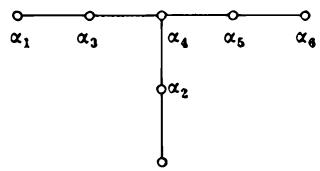
\includegraphics[keepaspectratio]{images/part002_9f0044a9.jpg}}

\begin{enumerate}
\def\labelenumi{(\Alph{enumi})}
\setcounter{enumi}{21}
\tightlist
\item
  由于 \((\alpha |\alpha) = 2\) 对所有 \(\alpha \in \mathbb{R}\) 成立，所以 \(\mathbb{R}^{\sim} = \mathbb{R}\) 。对于 \(\Phi_{\mathbb{R}}\) ，根的长度平方为 \(\frac{1}{12}\) ，因此
\end{enumerate}

\[
\Phi_ {\mathrm{R}} (x, y) = (x | y) / 24, \quad \text { and } \quad \gamma (\mathrm{R}) = 144.
\]

\begin{enumerate}
\def\labelenumi{(\Roman{enumi})}
\setcounter{enumi}{5}
\tightlist
\item
  计算基本权得到：
\end{enumerate}

\[
\begin{array}{l} \omega_ {1} = \frac {2}{3} (\varepsilon_ {8} - \varepsilon_ {7} - \varepsilon_ {6}) = \frac {1}{3} (4 \alpha_ {1} + 3 \alpha_ {2} + 5 \alpha_ {3} + 6 \alpha_ {4} + 4 \alpha_ {5} + 2 \alpha_ {6}) \\ \omega_ {2} = \frac {1}{2} (\varepsilon_ {1} + \varepsilon_ {2} + \varepsilon_ {3} + \varepsilon_ {4} + \varepsilon_ {5} - \varepsilon_ {6} - \varepsilon_ {7} + \varepsilon_ {8}) \\ \quad = \alpha_ {1} + 2 \alpha_ {2} + 2 \alpha_ {3} + 3 \alpha_ {4} + 2 \alpha_ {5} + \alpha_ {6} = \tilde {\alpha} \\ \omega_ {3} = \frac {5}{6} (\varepsilon_ {8} - \varepsilon_ {7} - \varepsilon_ {6}) + \frac {1}{2} (- \varepsilon_ {1} + \varepsilon_ {2} + \varepsilon_ {3} + \varepsilon_ {4} + \varepsilon_ {5}) \\ \quad = \frac {1}{3} (5 \alpha_ {1} + 6 \alpha_ {2} + 10 \alpha_ {3} + 12 \alpha_ {4} + 8 \alpha_ {5} + 4 \alpha_ {6}) \\ \omega_ {4} = \varepsilon_ {3} + \varepsilon_ {4} + \varepsilon_ {5} - \varepsilon_ {6} - \varepsilon_ {7} + \varepsilon_ {8} \\ \quad = 2 \alpha_ {1} + 3 \alpha_ {2} + 4 \alpha_ {3} + 6 \alpha_ {4} + 4 \alpha_ {5} + 2 \alpha_ {6} \\ \omega_ {5} = \frac {2}{3} (\varepsilon_ {8} - \varepsilon_ {7} - \varepsilon_ {6}) + \varepsilon_ {4} + \varepsilon_ {5} \\ \quad = \frac {1}{3} (4 \alpha_ {1} + 6 \alpha_ {2} + 8 \alpha_ {3} + 12 \alpha_ {4} + 10 \alpha_ {5} + 5 \alpha_ {6}) \\ \omega_ {6} = \frac {1}{3} (\varepsilon_ {8} - \varepsilon_ {7} - \varepsilon_ {6}) + \varepsilon_ {5} \\ \quad = \frac {1}{3} (2 \alpha_ {1} + 3 \alpha_ {2} + 4 \alpha_ {3} + 6 \alpha_ {4} + 5 \alpha_ {5} + 4 \alpha_ {6}). \end{array}
\]

\begin{enumerate}
\def\labelenumi{(\Roman{enumi})}
\setcounter{enumi}{6}
\tightlist
\item
  正根之和的一半是 \(\sum_{i=1}^{6} \omega_i\) ，所以
\end{enumerate}

\[
\begin{array}{r l} \rho & = \varepsilon_ {2} + 2 \varepsilon_ {3} + 3 \varepsilon_ {4} + 4 \varepsilon_ {5} + 4 (\varepsilon_ {8} - \varepsilon_ {7} - \varepsilon_ {6}) \\ & = 8 \alpha_ {1} + 11 \alpha_ {2} + 15 \alpha_ {3} + 21 \alpha_ {4} + 15 \alpha_ {5} + 8 \alpha_ {6}. \end{array}
\]

\begin{enumerate}
\def\labelenumi{(\Roman{enumi})}
\setcounter{enumi}{7}
\tightlist
\item
  由第 10 号 (VIII) 及 § 1，第 10 号，命题 28，
\end{enumerate}

\[
\mathrm{Q} (\mathrm{R}) = \mathrm{Q} (\mathrm{R} _ {8}) \cap \mathrm{V} = \mathrm{L} _ {3} \cap \mathrm{V} \quad \text { and } \quad \mathrm{P} (\mathrm{R}) = p (\mathrm{P} (\mathrm{R} _ {8})) = p (\mathrm{L} _ {3}),
\]

其中 p 表示从 E 到 V 的正交投影。我们有

\[
p (\alpha_ {7}) = \alpha_ {7} - \frac {2}{3} \pi + \omega , \quad p (\alpha_ {8}) = \alpha_ {8} + \pi - 2 \omega .
\]

群 \(Q(R)\) 的基为 \((\alpha_{1},\ldots,\alpha_{6})\) 。群 \(P(R)\) 由 \(Q(R)\) 和 \(p(\alpha_{7})\) 生成，因为 \(p(\alpha_{8})\in P(R_{8})\cap V=Q(R_{8})\cap V=Q(R)\) 。我们有 \(3p(\alpha_{7})\in Q(R)\) 且 \(p(\alpha_{7})\notin Q(R)\) 。因此，群 \(P(R)/Q(R)\) 同构于 Z/3Z；例如，它由 \(\omega_{6}\) 的像生成。

连通指标为 3。

\begin{enumerate}
\def\labelenumi{(\Roman{enumi})}
\setcounter{enumi}{8}
\tightlist
\item
  (IX) 和 (X) 由 § 2，第 4 号，命题 7，Weyl 群的阶为 6!1.2.2.3.2.1.3 = \(2^{7}.3^{4}.5\) 。指数序列在 1 与 11 之间有 6 项，并包含与 12 互素的整数 1、5、7、11。其他指数 \(m, m'\) 是满足
\end{enumerate}

\[
m + m ^ {\prime} = 12.
\]

\[
(m + 1) \left(m ^ {\prime} + 1\right) (1 + 1) (5 + 1) (7 + 1) (11 + 1) = 2 ^ {7}. 3 ^ {4}. 5,
\]

根据第 V 章 § 6，第 2 号，公式 (2) 以及命题 3 的推论 1。第二个关系给出 \((m + 1)(m' + 1) = 45\) ，又因 \(m + m' + 2 = 14\) ，得到 \(m = 4\) ，\(m' = 8\) 。因此，指数序列为

\[
1, 4, 5, 7, 8, 11.
\]

\begin{enumerate}
\def\labelenumi{(\Roman{enumi})}
\setcounter{enumi}{10}
\tightlist
\item
  (XI) 和 (XII) 由于所有根的长度都相同，Dynkin 图的自同构就是底层图的自同构。除恒等自同构外，只有自同构 \(\varepsilon\) 将 \(\alpha_{1},\alpha_{3},\alpha_{4},\alpha_{5},\alpha_{6},\) \(\alpha_{2}\) 分别变为 \(\alpha_{6},\alpha_{5},\alpha_{4},\alpha_{3},\alpha_{1},\alpha_{2}\) 。因此，\(\mathrm{A(R) / W(R)}\) 同构于 \(\mathbf{Z} / 2\mathbf{Z}\) ；由于 \(-1\in \mathrm{W(R)}\) （第 V 章 §6，第 2 号，命题 3 的推论 3），\(\mathrm{A(R)}\) 同构于 \(\mathrm{W(R)}\times \{1, - 1\}\) ，且可将 \(w_0\) 认作 \(-\varepsilon\) 。由此，\(\mathrm{A(R) / W(R)}\) 的非恒等元素定义了自同构 \(x\mapsto -x\)，该自同构作用于 \(\mathrm{P(R^{\prime}) / Q(R^{\prime})}\)。
\end{enumerate}

此外，\(P(R^{-})/Q(R^{-})\) 有两个阶为 3 的非恒等元素。它们定义了扩充 Dynkin 图的两个三阶自同构。

